\subsection{Huffmancodes}

Huffmancodes worden opgeslagen in de vorm van onderstaande \emph{struct}. De codes worden bijgehouden in de bladeren van de boom, al koos ik ervoor dit enkel te doen bij het Standaard Huffmancoding-algoritme en niet bij de andere vier algoritmes. De reden hiervoor is dat aangezien bij de andere vier algoritmes de codes veranderen tijdens het encoderen/decoderen, waardoor de codes ook zouden moeten bijgewerkt worden.
\begin{figure}[h]
	\centering
	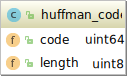
\includegraphics[width=10em]{resources/huffman-code.png}
	\caption{Huffman code}
\end{figure}
\\Het veld \emph{length} bevat de lengte van de code en \emph{code} bevat de eigenlijke code. Theoretisch kan de maximale lengte van een Huffmancode $255$ bits bedragen. De bekomen Huffmanboom heeft dan een maximale diepte.
\begin{figure}[h]
	\centering
\begin{tikzpicture}[-,>=stealth',level/.style={sibling distance = 5cm/#1,
	level distance = 1.5cm},scale=0.6, transform shape]
\node[treenode] {root}
child
{
	node [treenode] {}
	child
	{
		node [treenode] {}
		child
		{
			node [treenode] {}
			child
			{
				node [treenode] {$255$}
			}
			child
			{
				node [treenode] {$254$}
			}
		}
		child
		{
			node [treenode] {$002$}
		}
	}
	child
	{
		node [treenode] {$001$}
	}
}
child
{
	node [treenode] {$000$}
}
;
\end{tikzpicture}
\caption{Huffmanboom met maximale diepte}
\end{figure}
\\Bovenstaande boom kan enkel voorkomen als de frequenties van de karakters verdeeld zijn volgens de reeks van Fibonacci, immers, het algoritme dat de Huffmanboom opbouwt kiest telkens de 2 Huffmanbomen met het kleinste gewicht en voegt deze samen. Bij een Fibonacci-verdeling zal het algoritme dus steeds de reeds bestaande Huffmanboom samenvoegen met een volgend karakter. De samengevoegde Huffmanboom zal als gewicht steeds de som van het nieuwe karakter en de reeds bestaande Huffmanboom krijgen, wat exact gelijk is aan het gewicht van het volgende karakter dat zou worden toegevoegd, wegens de definitie van de Fibonacci-reeks. Een code die langer is dan 64 bits kan dus enkel voorkomen als de frequenties van de inputreeks Fibonacci verdeeld zijn tot minstens het 64\textsuperscript{e} Fibonacci getal. De minimale grootte van deze tekst kan berekend worden met onderstaande formule. Aangezien bij Standaard Huffmancoding deze tekst in 1 keer in het \emph{RAM}-geheugen moet passen, is het niet nodig om codes langer dan 64 bits te ondersteunen.
\begin{figure}[h]
	$$l = \sum_{i=1}^{64} fib(i)\text{, met }fib(x) = fib(x-1) + fib(x-2)\text{ en }fib(0) = fib(1) = 1$$
	\caption{Minimale codelengte}
\end{figure}